% https://pxl-digital.pxl.be/page/seminarie-aarixa-27-02

Mijn eerste seminarie ging over Docker, een tool om applicaties in containers te runnen. De spreker Sven Luts, software engineer bij AariXa, kwam uitleggen wat deze tool is, waarom het gebruikt wordt en hoe het achterliggend werkt aan de hand van demo's.

Als aller eerste stelde de spreker zich voor, hij vertelde waar hij werkte, wat zijn hobby's waren en wat zijn specialiteiten zijn op gebied van informatica. Dan begon de introductie van Docker, het is een tool gemaakt om het versimpelen van het aanmaken, deployen en runnen van applicaties gebruik makend van containers.

Het volgende onderdeel ging over waarom je Docker moet gebruiken. Het vereenvoudigd het maken en deployen van software, het is veel sneller dan dan virtuele machines, heeft ingebouwde version tracking en het voorkomt de gekende uitspraak: "It works on my machine". Omdat het in een afgeschermde en geïsoleerde omgeving is, hoef je geen rekening te houden met reeds geïnstalleerde dependencies of conflicterende dependencies. Door gebruik te maken van Docker tags, heb je al een ingebouwde versie tracking. En omdat de container op eender welke computer kan runnen en iedere keer exact hetzelfde zal reageren en dezelfde dependencies hebben.

Daarna vertelde de spreker wat Docker containers zijn, hoe je ze kan maken of afhalen van het internet. Een container kan vergeleken worden met een virtuele machine, in de zin dat het ge\"isoleerd is van de host computer en dat het alles bevat wat de applicatie nodig heeft om te runnen. Maar in tegenstelling tot een virtuele machine gaat een Docker container het operating system niet virtualiseren, maar het gebruikt die van de host. Hierdoor wordt de container veel kleiner dan een virtuele machine en heeft het praktisch geen opstarttijd.

De containers kunnen zelf gemaakt worden aan de hand van Dockerfiles waarin het build proces van een image gedefinieerd wordt. Er kunnen ook images afgehaald worden van een hub of repository door deze te pullen. Als er een image is, door ze te builden of pullen, kan hier een container van opgestart worden door de image te runnen. Er kunnen meerdere containers runnen van eenzelfde image. Na wijzigingen kan de container terug opgeslagen worden als een image en eventueel gepusht worden naar een repository of hub.

Na deze uitleg toonde Sven Luts ons hoe we Docker zelf konden installeren. Voor Docker werd er vooral met Linux gewerkt, als je het op Mac of Windows wou installeren draaide je achterliggend een Linux virtuele machine waarin je je containers kon draaien. Na de installatie volgde de basis commando's om de voordien uitgelegde acties uit te voeren en commando's om Docker te beheren en monitoren.

Als afsluiter kregen we een demo te zien hoe snel en makkelijk Docker is een een website waar we dit zelf konden proberen zonder dat er een installatie nodig was. Dit was eerder de Hello World van Docker. En hij gaf een kleine vooruitblik naar wat er in de toekomst met Docker kan gebeuren en gerealiseerd worden. Zoals redundancy, load balancing, health monitoring en nog veel meer.

\begin{figure}[!h]
  \centering
  \begin{subfigure}[h]{0.37\textwidth}
    \centering
    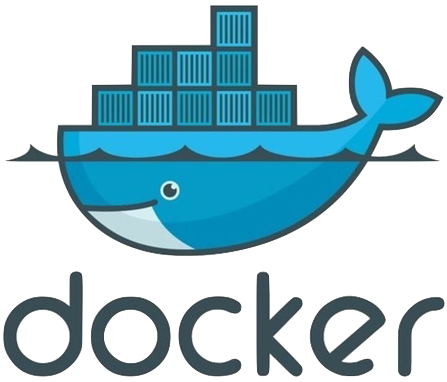
\includegraphics[width=0.8\linewidth]{docker/logo.png}
  \end{subfigure}
  \begin{subfigure}[h]{0.59\textwidth}
    \centering
    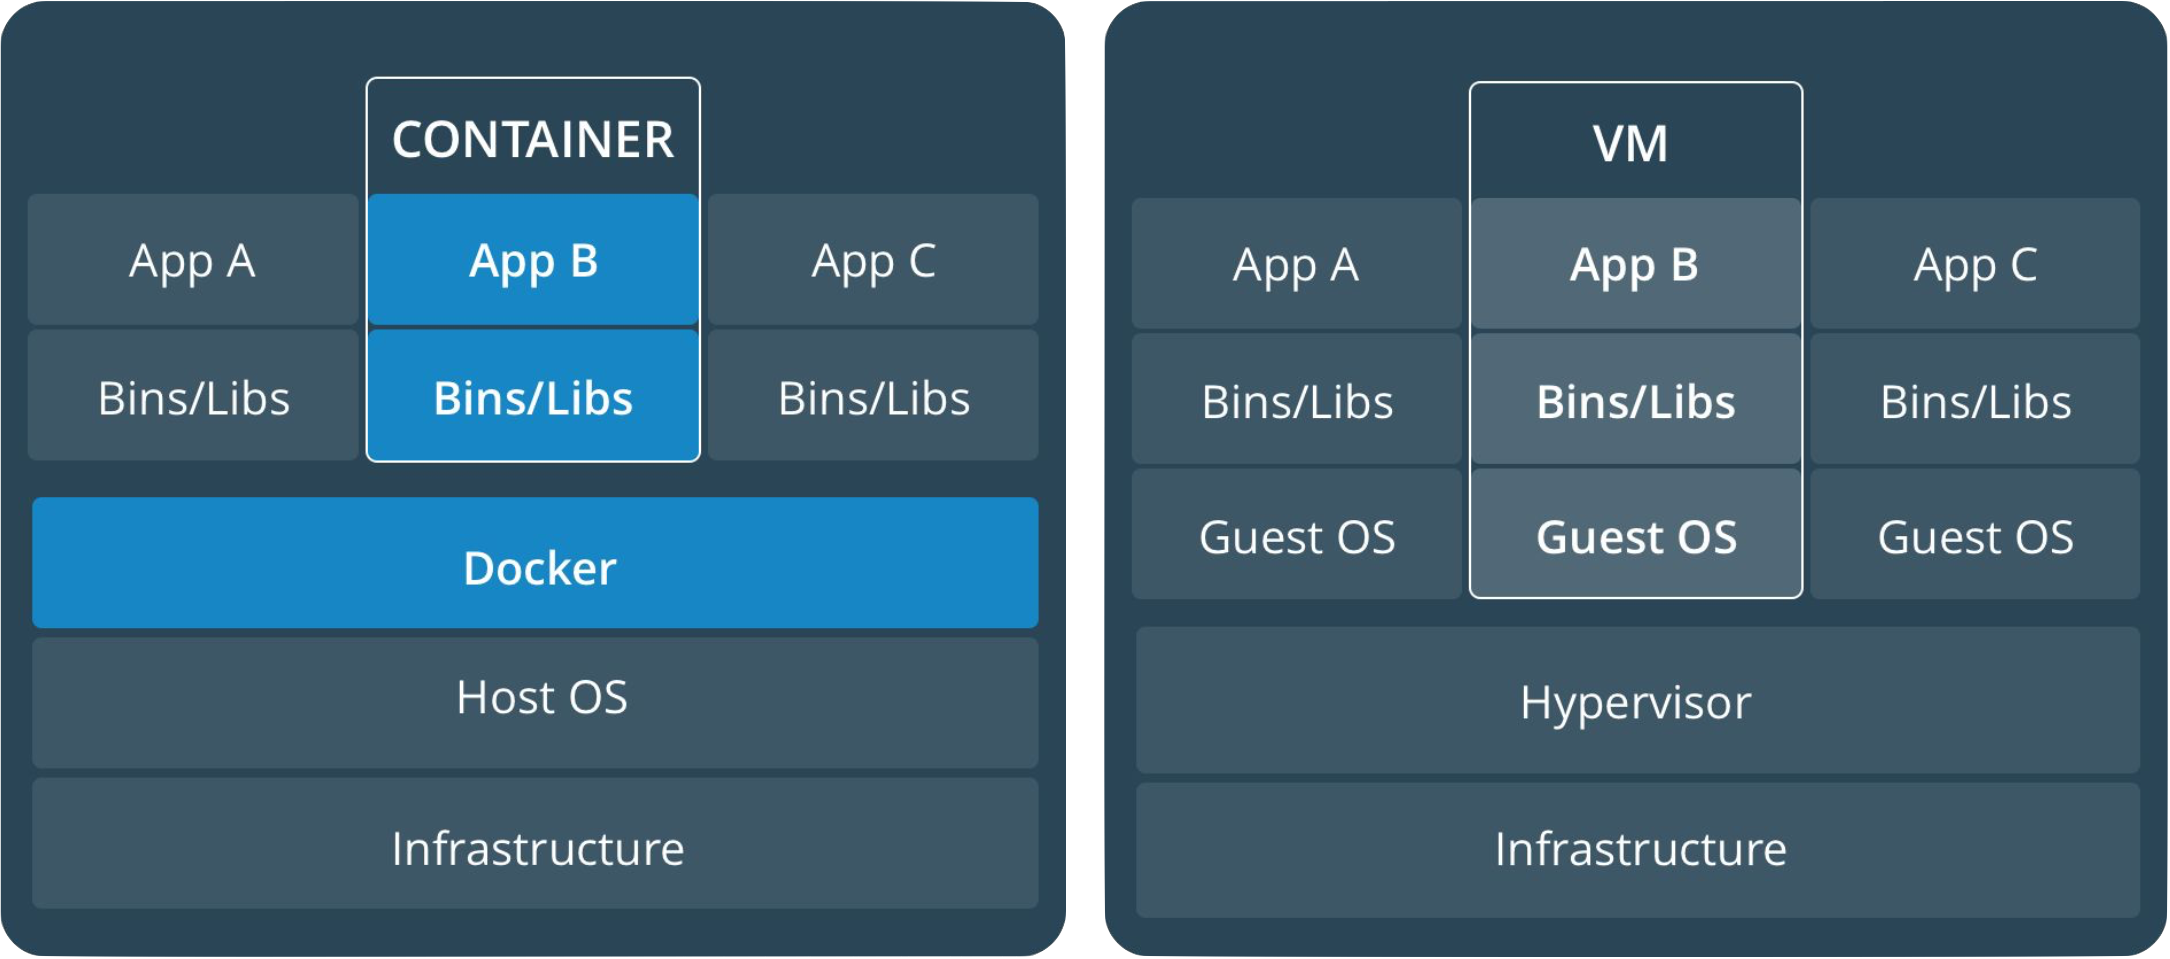
\includegraphics[width=\linewidth]{docker/docker_vs_vm.png}
  \end{subfigure}
\end{figure}

Initieel vond ik het onderwerp van het seminarie boeiend, maar kon ik niet plaatsen hoe ik deze technologie zou kunnen gebruiken binnen mijn toekomstige projecten. Echter, toen ik gedurende de vakken rond artifici\"ele intelligentie en robotica in aanraking kwam met Docker, zag ik het het nut van dit seminarie in. Dit gaf mij niet alleen een grote voorsprong op mijn medestudenten die hier nog niet mee in aanraking gekomen waren, maar het deed mij ook beseffen dat het een zeer praktische technologie is waar ik in de toekomst ook nog gebruik van zou kunnen maken.

Ondertussen heb ik al meerdere projecten met en in Docker gemaakt, ook mijn IT\hyp{}project en stage hadden Docker als basis. Dit seminarie en deze technologie hebben mij ge\"inspireerd om ge\"isoleerde applicaties te schrijven, maar ook hoe ik met dependencies kan en moet omgaan. Docker heeft mij ook al zeer veel tijd uitgespaard door het feit dat je meer kan experimenteren en altijd kan terugvallen op een punt waar de applicatie werkend is zonder enige moeite.

De spreker bracht deze presentatie zeer rustig en haalde goede punten aan. Hij verloor onze aandacht niet door niet af te dwalen, maar leuke weetjes over het huidige onderwerp kon aanbrengen. Zijn eigen ervaringen met Docker waren zeer leuke projecten dat volgens hem relatief snel ontwikkeld konden worden.

Ik ben zeer blij dat ik dit seminarie heb opgenomen omwille van het gebruik van Docker nu, maar het is zeker nuttig voor iedereen om te weten wat deze technologie is en het te overwegen om deze zelf te gebruiken. Naar mijn mening, mag Docker ook gegeven of aangehaald worden in vakken zoals Desktop OS of Server OS Essentials.

Spreker: Sven Luts, software engineer bij AariXa, \url{https://be.linkedin.com/in/svenluts/nl}


\begin{figure}[!h]
  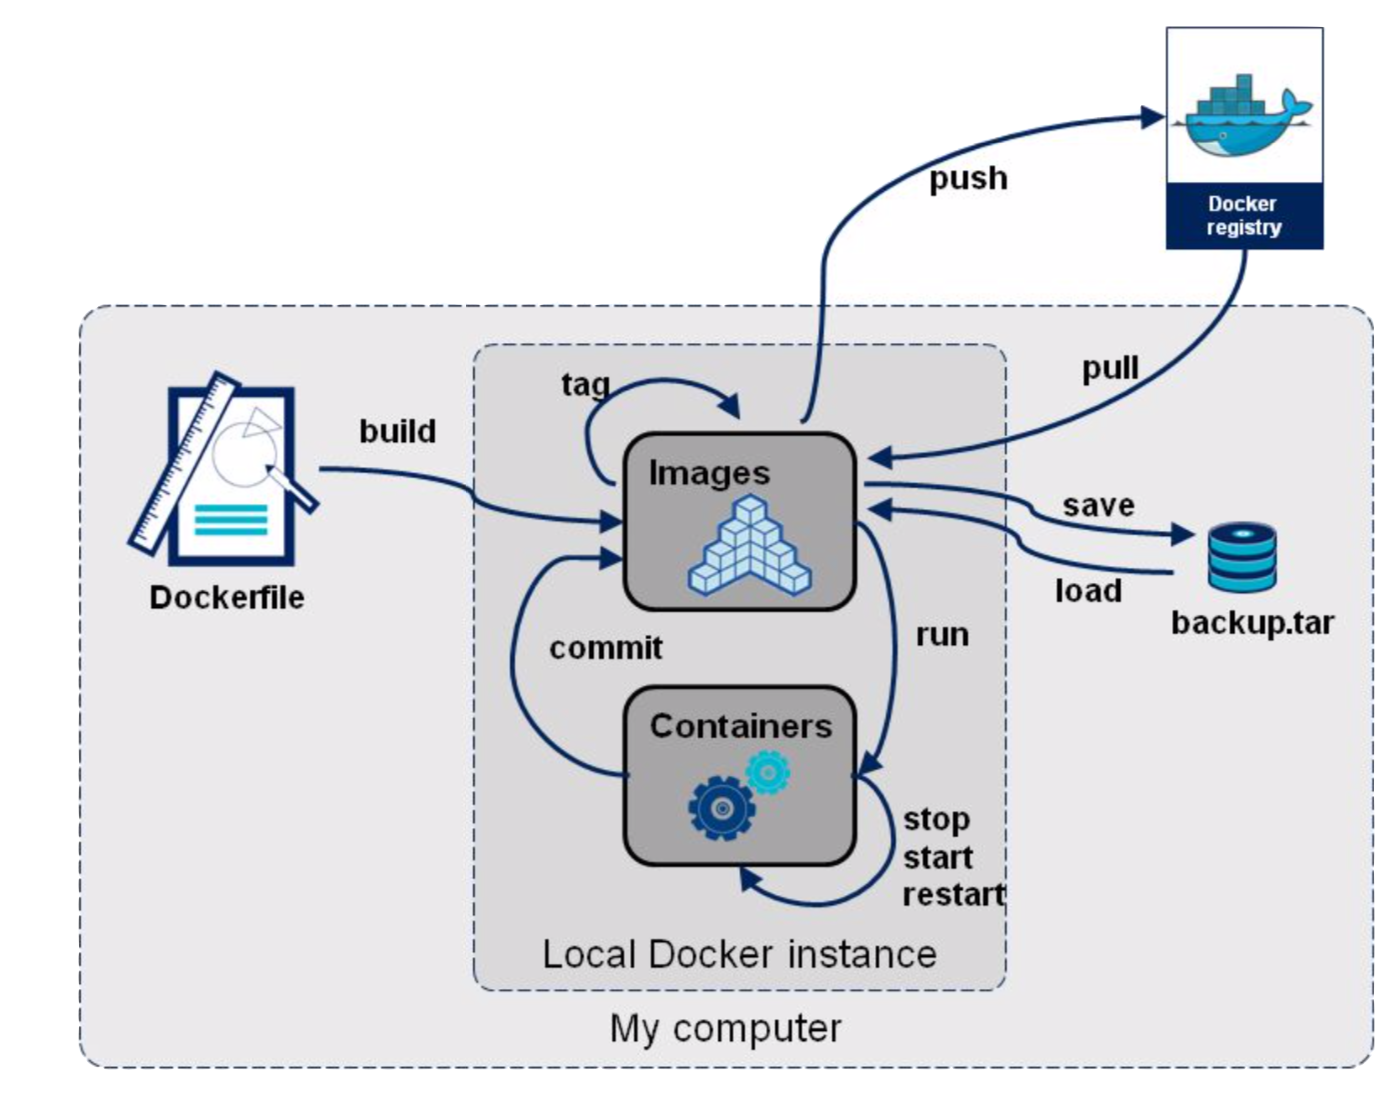
\includegraphics[width=\linewidth]{docker/flow.png}
\end{figure}